 \documentclass{article}

% cursor parking lot please place 
% your cursor here when you go away
% so other's can work :) 
% -------------------------
% |     |     |     |     |
% |     |     |     |     |
% -------------------------

% libraries
\usepackage{amsmath, amssymb, hyperref, fullpage, enumitem, graphicx, subcaption, float, braket} 

% code blocks
\usepackage[most]{tcolorbox}
\usepackage{minted}

\tcbset{
  codebox/.style={
    listing engine=minted,
    colback=gray!10,
    colframe=gray!40,
    boxsep=4pt,
    arc=2pt,
    outer arc=2pt,
    top=2pt, bottom=2pt, left=4pt, right=4pt,
    listing only,
    breakable,
    fonttitle=\scriptsize\bfseries,
    coltitle=black,
    colbacktitle=gray!20,
    minted options={
      linenos=false,
      breaklines=true,
      fontsize=\small,
      autogobble=true
    },
  }
}

\newtcblisting{python}{
  codebox,
  title=Python,
  minted language=python,
}

\newtcblisting{rcode}{
  codebox,
  title=R,
  minted language=r,
}

% ignore these ... 
\setlength{\parindent}{0pt}
\setlength{\parskip}{\medskipamount}
\setcounter{secnumdepth}{-2}

\begin{document}

These notes follow: \href{https://arxiv.org/pdf/1606.02950}{``Lectures on the Bethe Ansatz"}, and is produced by Esha Sury and Dhruv Upreti.

\section{Bethe Ansatz Theory}

The \href{https://en.wikipedia.org/wiki/Bethe_ansatz}{Bethe Ansatz}, is a collection of methods used to obtain exact solutions to certain \href{https://en.wikipedia.org/wiki/Many-body_problem}{quantum many-body systems}, especially one-dimensional quantum \href{https://en.wikipedia.org/wiki/Integrable_system}{integrable models}. In favorable cases, the Bethe Ansatz gives the exact energy spectrum and corresponding eigenstates by reducing the many-body eigenvalue problem to a set of algebraic equations called the \textbf{Bethe equations}. 

Intuitively, in models solvable by the Bethe Ansatz, many body scattering is \textbf{non-diffractive} meaning that particles retain their individual momenta after collisions, and the full many body scattering matrix factorizes into an ordered product of two body \href{https://en.wikipedia.org/wiki/S-matrix}{scattering matrices}. The \href{https://en.wikipedia.org/wiki/Yang%E2%80%93Baxter_equation}{Yang Baxter equation} is the consistency condition ensuring that the different possible orders in which the same many body scattering process can be decomposed into two body scatterings give equivalent results.

\subsection{Asymptotic Bethe Ansatz Equations in 1+1 Dimensional Quantum Field Theory}

This section discuss the Bethe equations for the spectrum of a generic $1+1$ dimensional integrable theory. We consider a theory on a circle, line segment of length $L$ with periodic boundary conditions. In an integrable theory the scattering has features highlighted above: 

\begin{itemize}
    \item The number of particles is conserved in any scattering event.
    \item The momenta do not change but can only be redistributed between particles.
    \item The $S$-matrix for multiparticle scattering factorizes; this means the $S$-matrix for any number of particles is a product of the $2\to 2$ $S$ matrices.
\end{itemize}

Starting with a toy model, a theory with only one particle in its particle spectrum of the QFT, such as the \href{https://en.wikipedia.org/wiki/Sine-Gordon_equation}{sinh-Gordon model} for some values of the parameters.

Recall from quantum mechanics, \href{https://en.wikipedia.org/wiki/Momentum_operator}{momentum} is the generator of spatial translations since $\hat{p} = -i d/dx$ (for $\hbar = 1$), then the eigenvalue equation becomes $\hat{p}\,\psi(x) = p\,\psi(x) \Rightarrow \psi(x) = Ce^{ipx}$. Therefore a particle with definite momentum $p$ should have the property that if you translate it by a distance $a$, it only changes by a phase, 

\[\psi(x+a) = e^{ipa}\psi(x).\]

Imagine the first particle is taken around the circle once, eventually bringing it back to its place again. If there w`ere no other particles (or if the theory was non-interacting) the wavefunction would acquire a phase factor $e^{ip_1 L}$, and by the periodicity of the system $e^{ip_1 L} = 1$ so $p_1 = 2\pi k/L$ for $k\in\mathbb{Z}$. 

\begin{figure}[H]
    \centering
    \begin{subfigure}[b]{0.4\linewidth}
        \centering
        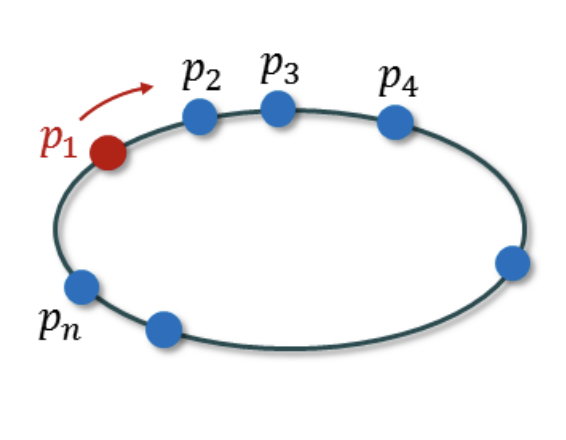
\includegraphics[width=\linewidth]{figures/particles_on_circle.png}
        \caption{Deriving the periodicity condition on a circle. We take the first particle with momentum $p_1$ around the circle, scattering it through all the other particles.}
    \end{subfigure} \hfill
    \begin{subfigure}[b]{0.4\linewidth}
        \centering
    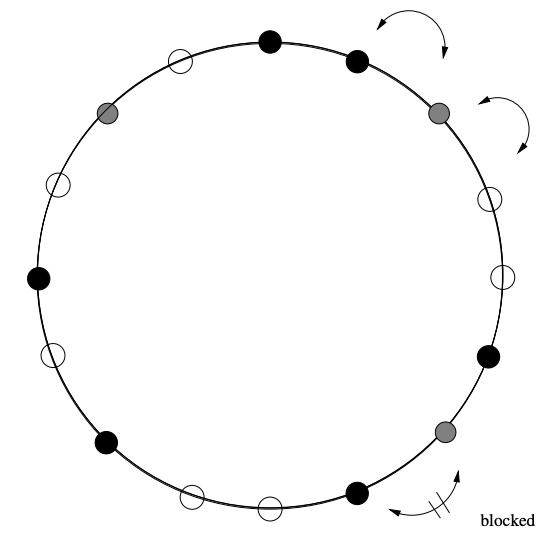
\includegraphics[width=\linewidth]{figures/asym_diffusion_on_ring.png}
        \caption{}
    \end{subfigure}
    \caption{}
\end{figure}

Taking into account the interaction with other particles, if $L$ is large compared to the interaction range between the particles the interaction is described by the asymptotic $S$-matrix (which is just the $S$-matrix defined using particles that are infinitely far apart before and after scattering since each collision looks approximately like an ordinary infinite line scattering event), for a one particle species integrable theory, the two particle asymptotic $S$-matrix is just a phase, 

\[S(p_1, p_2) = e^{i\alpha(p_1,p_2)}.\] 

This is due to the fact that in this toy model with only one particle type in the spectrum and the theory is integrable the number of particles is conserved and the momenta cannot change except possibly being exchanged, so after scattering it only gains a complex phase, 

\[\ket{p_1,p_2}_{\text{out}} = S(p_1, p_2)\,\ket{p_1, p_2}_{\text{in}}, \quad |S(p_1, p_2)| = 1 \text{ so } S(p_1, p_2) = e^{i\alpha(p_1, p_2)}.\]

When we take the particle around the circle it will scatter through all other particles as shown in Figure 1(a) so we see that,

\[e^{ip_1 L} S(p_1,p_2)S(p_1,p_3)\cdots S(p_1,p_n) = 1\]

For any particle we get,

\[e^{ip_jL}\prod_{k=1,k\neq j}^n S(p_j,p_k) = 1, \quad \text{asymptotic Bethe Ansatz equations}\]

This is a set of $n$ algebraic equations for $n$ variables $p_1\cdots p_n$ which allows us to fix the values of the momenta. In regions where the particles are well separated they propagate freely, so the energy of the state should always be equal to simply the sum of individual particles’ energies given as,

\[E = \sum_i \varepsilon(p_i).\]

Note that the asymptotic Bethe equations only describes the energy in a large volume $L$, more precisely the Bethe equations capture all terms in the large $L$ expansion of the energy which scale as $\sim 1/L^k$ known as the powerlike corrections but miss exponential corrections of the kind $\sim e^{-mL}$ ($m$ is the particle's mass) which physically correspond to the effects of virtual particles propagating around the circle. % Note i need to get a better explanation for this since i dont understand this all that well 





\section{Example: 1D Spin-1/2 Heisenberg Chain}

This section follows: \href{https://homepages.dias.ie/dorlas/Papers/Bethe.pdf}{``On the Theory of Metals. I. Eigenvalues and Eigenfunctions of the Linear Atomic Chain"}, following Bethe's original formulation of the ansatz for a 1D metal consisting of a linear chain of atoms, each of which has a single $s$ electron with spin.

\end{document}